\section{Понятие естественного отбора}

\indent \indentПроцесс естественного отбора начинается с выбора наиболее приспособленных особей из популяции. Они производят потомство, которое наследует характеристики родителей и будет добавлено к следующему поколению. Если родители подготовлены лучше, то их дети имеют больше шансов на выживание. Этот процесс продолжает повторяться, и в конце, поколение с самыми подходящими особями будет найдено.

Это понятие может быть применено к проблеме обучения нейронной сети. В работе рассматривается набор решений для проблемы и выбирается из них набор лучших.

\subsubsection{Пять фаз эволюционного алгоритма}
\begin{itemize}
  \item Начальная популяция;
  \item фитнес-функция;
  \item выбор;
  \item скрещивание;
  \item мутация.
\end{itemize}

\subsubsection{Начальная популяция}
\indent \indent Процесс начинается с набора нейронный сетей. Каждая нейроная сеть(индивидуум) умеет решать поставленную задачу с каким-то уровнем успеха.
Индивидуум характеризуется набором параметров (переменных), известных как гены. Гены объединяются в цепочку, образуя хромосому.

В эволюционном алгоритме набор генов индивида представлен строкой в алфавитном порядке. Обычно используются двоичные значения (строка из 1 и 0). Часто говорят, что таким образом кодируются гены в хромосоме.

\subsubsection{Фитнес-функция}
\indent \indent Функция пригодности(финтес-функция) определяет, насколько подходит индивидуум(способность нейросети конкурировать с другими нейронными сетями) для решения конкретной задачи. Это дает оценку пригодности для каждой сети. Вероятность того, что конкретная нейронная сеть будет выбрана для скрещивания, основана на ее оценке пригодности.

Идея фазы отбора состоит в том, чтобы отобрать наиболее подходящих особей и позволить им передать свои гены следующему поколению. Две пары индивидуумов (родителей) выбираются на основе их показателей пригодности. Нейронный сети с высоким процентом ответов имеют больше шансов быть отобранными для размножения.

\subsubsection{Скрещивание}
\indent \indent Скрещивание является наиболее значимой фазой в генетическом алгоритме. Для каждой пары родителей, которые должны быть спарены, точка пересечения(crossover point) выбирается случайным образом из генов.
Например, рассмотрим точку пересечения 3, как показано ниже (рис 2.1). 

\begin{figure}[H]
  \centering
  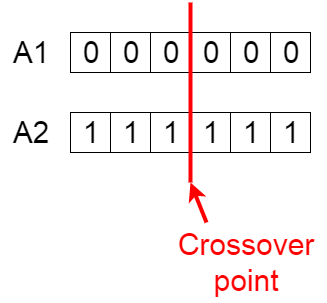
\includegraphics[width=0.4\linewidth]{./img/crossover-point}
  \caption{Точка пересечения(crossover point)}
  \label{fig:mpr}
\end{figure} 

Потомки создаются путем обмена генами родителей между собой, пока не будет достигнута точка пересечения.

\begin{figure}[H]
  \centering
  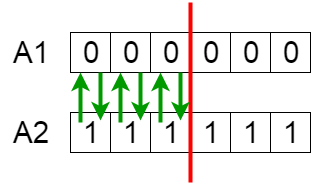
\includegraphics[width=0.4\linewidth]{./img/genesis}
  \caption{Обмен генами}
  \label{fig:mpr}
\end{figure} 

В итоге получается новое потомство.

\begin{figure}[H]
  \centering
  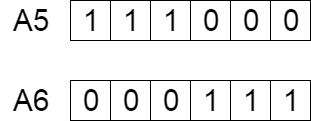
\includegraphics[width=0.4\linewidth]{./img/child}
  \caption{Потомки}
  \label{fig:mpr}
\end{figure}

\subsubsection{Мутация}
У некоторых новых потомков отдельные  гены могут подвергаться мутации с низкой случайной вероятностью. Это подразумевает, что некоторые биты в битовой строке могут быть перевернуты.

\begin{figure}[H]
  \centering
  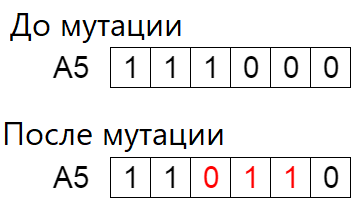
\includegraphics[width=0.4\linewidth]{./img/mutation}
  \caption{Мутация}
  \label{fig:mpr}
\end{figure}

\indent \indent Мутация происходит для поддержания разнообразия в популяции и предотвращения преждевременной конвергенции. Алгоритм завершается, если популяция не производит потомство, которое значительно отличается от предыдущего поколения.